\documentclass[14pt]{extbook}
\usepackage{multicol, enumerate, enumitem, hyperref, color, soul, setspace, parskip, fancyhdr} %General Packages
\usepackage{amssymb, amsthm, amsmath, bbm, latexsym, units, mathtools} %Math Packages
\everymath{\displaystyle} %All math in Display Style
% Packages with additional options
\usepackage[headsep=0.5cm,headheight=12pt, left=1 in,right= 1 in,top= 1 in,bottom= 1 in]{geometry}
\usepackage[usenames,dvipsnames]{xcolor}
\usepackage{dashrule}  % Package to use the command below to create lines between items
\newcommand{\litem}[1]{\item#1\hspace*{-1cm}\rule{\textwidth}{0.4pt}}
\pagestyle{fancy}
\lhead{Progress Quiz 10}
\chead{}
\rhead{Version C}
\lfoot{6232-9639}
\cfoot{}
\rfoot{Fall 2020}
\begin{document}

\begin{enumerate}
\litem{
Solve the radical equation below. Then, choose the interval(s) that the solution(s) belongs to.\[ \sqrt{21 x^2 + 10} - \sqrt{-29 x} = 0 \]\begin{enumerate}[label=\Alph*.]
\item \( x_1 \in [-0.72, -0.71] \text{ and } x_2 \in [-1.4,0.4] \)
\item \( \text{All solutions lead to invalid or complex values in the equation.} \)
\item \( x_1 \in [0.65, 0.67] \text{ and } x_2 \in [0,1.3] \)
\item \( x \in [-0.69,-0.66] \)
\item \( x \in [-0.72,-0.71] \)

\end{enumerate} }
\litem{
Solve the radical equation below. Then, choose the interval(s) that the solution(s) belongs to.\[ \sqrt{20 x^2 + 36} - \sqrt{-61 x} = 0 \]\begin{enumerate}[label=\Alph*.]
\item \( x_1 \in [-3.8, -1] \text{ and } x_2 \in [-3.8,0.2] \)
\item \( x \in [-1.4,0.2] \)
\item \( x \in [-3.8,-1] \)
\item \( x_1 \in [-0.2, 1] \text{ and } x_2 \in [2.25,4.25] \)
\item \( \text{All solutions lead to invalid or complex values in the equation.} \)

\end{enumerate} }
\litem{
Choose the graph of the equation below.\[ f(x) = - \sqrt[3]{x - 8} - 5 \]\begin{enumerate}[label=\Alph*.]
\begin{multicols}{2}\item 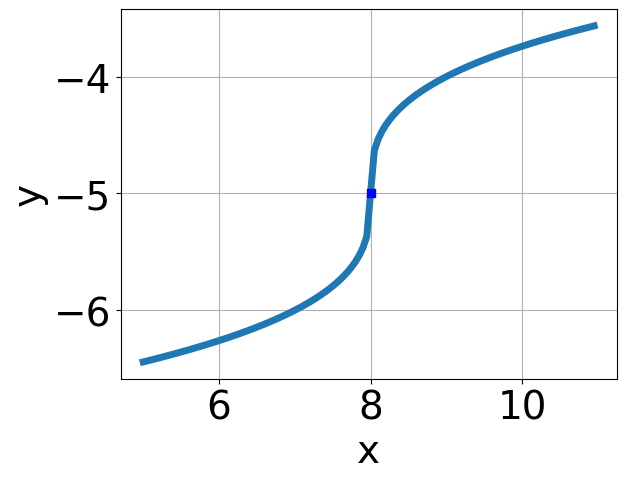
\includegraphics[width = 0.3\textwidth]{../Figures/radicalEquationToGraphCopyAC.png}\item 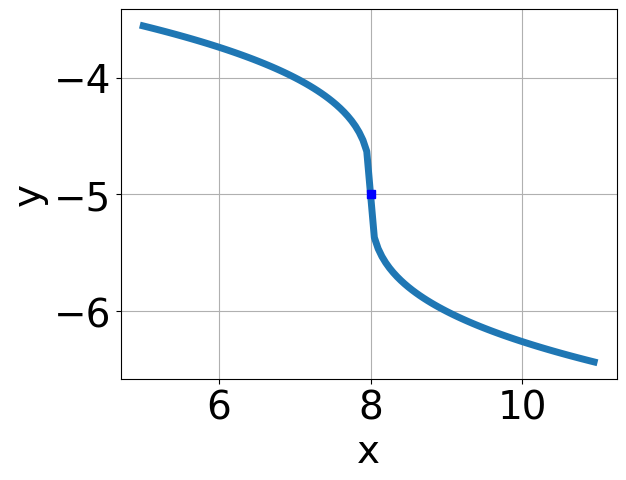
\includegraphics[width = 0.3\textwidth]{../Figures/radicalEquationToGraphCopyBC.png}\item 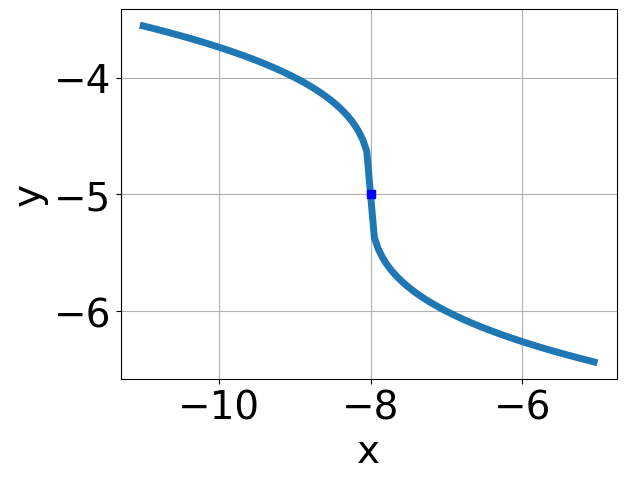
\includegraphics[width = 0.3\textwidth]{../Figures/radicalEquationToGraphCopyCC.png}\item 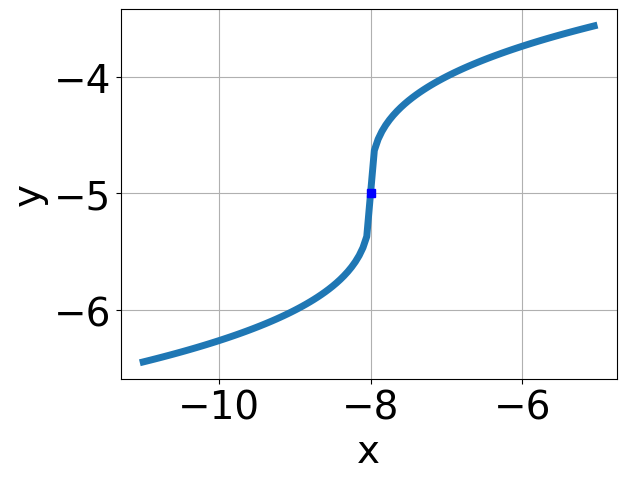
\includegraphics[width = 0.3\textwidth]{../Figures/radicalEquationToGraphCopyDC.png}\end{multicols}\item None of the above.
\end{enumerate} }
\litem{
What is the domain of the function below?\[ f(x) = \sqrt[6]{-9 x + 8} \]\begin{enumerate}[label=\Alph*.]
\item \( [a, \infty), \text{where } a \in [0.95, 1.35] \)
\item \( (-\infty, a], \text{where } a \in [0.97, 1.67] \)
\item \( [a, \infty), \text{where } a \in [0.56, 0.99] \)
\item \( (-\infty, a], \text{ where } a \in [0.02, 1.1] \)
\item \( (-\infty, \infty) \)

\end{enumerate} }
\litem{
Choose the graph of the equation below.\[ f(x) = - \sqrt{x - 8} - 6 \]\begin{enumerate}[label=\Alph*.]
\begin{multicols}{2}\item 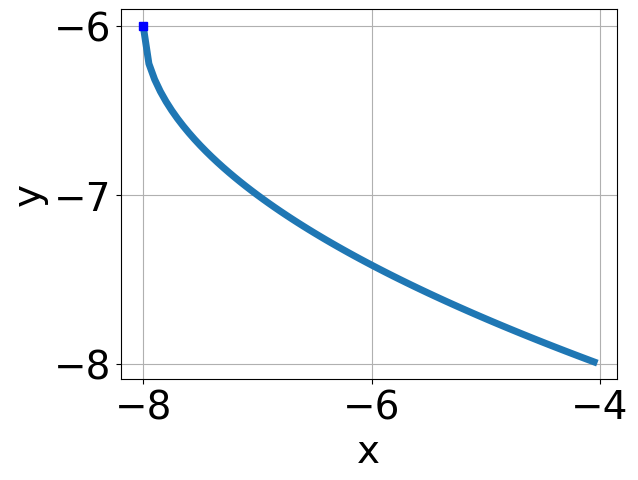
\includegraphics[width = 0.3\textwidth]{../Figures/radicalEquationToGraphAC.png}\item 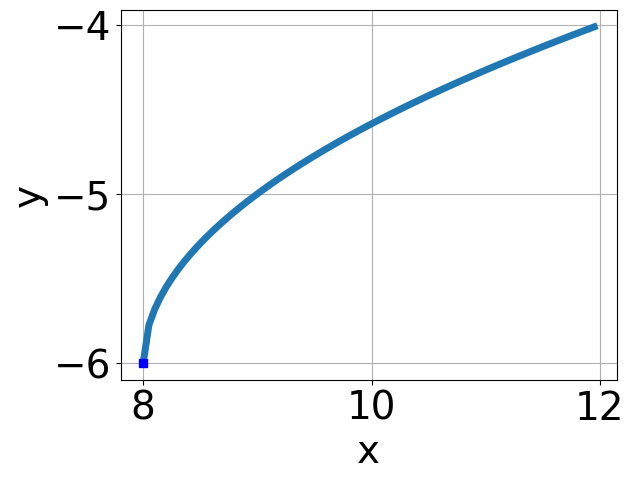
\includegraphics[width = 0.3\textwidth]{../Figures/radicalEquationToGraphBC.png}\item 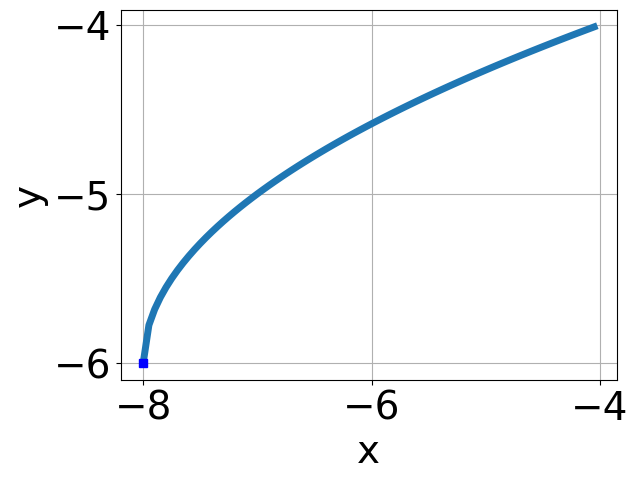
\includegraphics[width = 0.3\textwidth]{../Figures/radicalEquationToGraphCC.png}\item 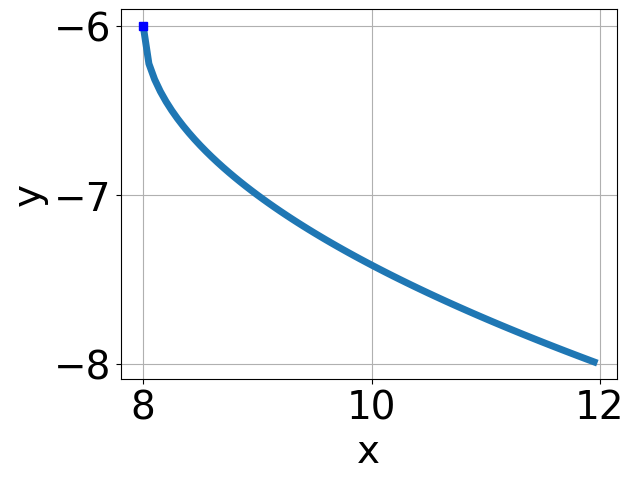
\includegraphics[width = 0.3\textwidth]{../Figures/radicalEquationToGraphDC.png}\end{multicols}\item None of the above.
\end{enumerate} }
\litem{
Choose the equation of the function graphed below.
\begin{center}
    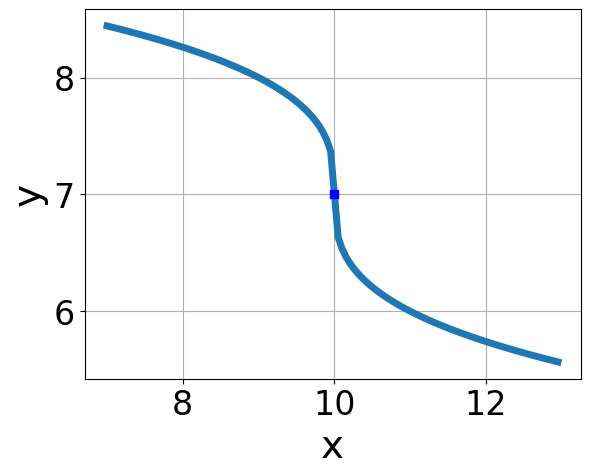
\includegraphics[width=0.5\textwidth]{../Figures/radicalGraphToEquationC.png}
\end{center}
\begin{enumerate}[label=\Alph*.]
\item \( f(x) = - \sqrt{x + 10} + 7 \)
\item \( f(x) = \sqrt{x - 10} + 7 \)
\item \( f(x) = \sqrt{x + 10} + 7 \)
\item \( f(x) = - \sqrt{x - 10} + 7 \)
\item \( \text{None of the above} \)

\end{enumerate} }
\litem{
Solve the radical equation below. Then, choose the interval(s) that the solution(s) belongs to.\[ \sqrt{-2 x + 2} - \sqrt{-9 x - 7} = 0 \]\begin{enumerate}[label=\Alph*.]
\item \( x_1 \in [-1.16, -0.17] \text{ and } x_2 \in [-6,6] \)
\item \( x_1 \in [-1.42, -1.05] \text{ and } x_2 \in [-6,6] \)
\item \( \text{All solutions lead to invalid or complex values in the equation.} \)
\item \( x \in [-1.42,-1.05] \)
\item \( x \in [0.48,0.82] \)

\end{enumerate} }
\litem{
Solve the radical equation below. Then, choose the interval(s) that the solution(s) belongs to.\[ \sqrt{-5 x + 5} - \sqrt{8 x - 8} = 0 \]\begin{enumerate}[label=\Alph*.]
\item \( \text{All solutions lead to invalid or complex values in the equation.} \)
\item \( x \in [-1.23,0.77] \)
\item \( x \in [1,4] \)
\item \( x_1 \in [1, 4] \text{ and } x_2 \in [1,2] \)
\item \( x_1 \in [1, 4] \text{ and } x_2 \in [1,2] \)

\end{enumerate} }
\litem{
What is the domain of the function below?\[ f(x) = \sqrt[8]{9 x + 6} \]\begin{enumerate}[label=\Alph*.]
\item \( (-\infty, a], \text{where } a \in [-2.53, -1.09] \)
\item \( [a, \infty), \text{where } a \in [-1.98, -1.19] \)
\item \( (-\infty, \infty) \)
\item \( (-\infty, a], \text{where } a \in [-0.9, -0.6] \)
\item \( [a, \infty), \text{ where } a \in [-1.45, 0.18] \)

\end{enumerate} }
\litem{
Choose the equation of the function graphed below.
\begin{center}
    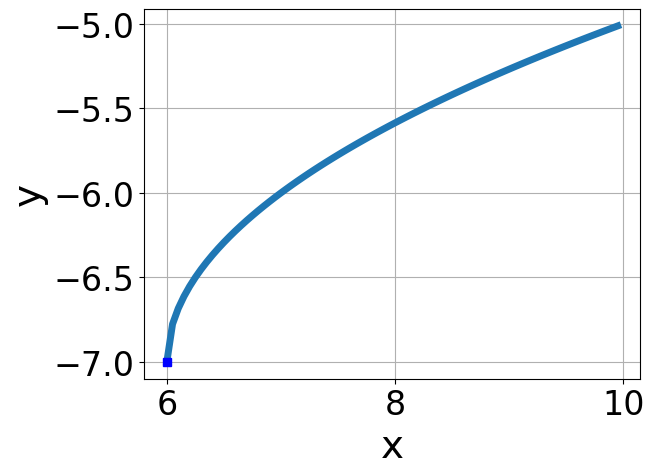
\includegraphics[width=0.5\textwidth]{../Figures/radicalGraphToEquationCopyC.png}
\end{center}
\begin{enumerate}[label=\Alph*.]
\item \( f(x) = \sqrt{x + 6} - 7 \)
\item \( f(x) = - \sqrt{x - 6} - 7 \)
\item \( f(x) = - \sqrt{x + 6} - 7 \)
\item \( f(x) = \sqrt{x - 6} - 7 \)
\item \( \text{None of the above} \)

\end{enumerate} }
\end{enumerate}

\end{document}